% Format teze zasnovan je na paketu memoir
% http://tug.ctan.org/macros/latex/contrib/memoir/memman.pdf ili
% http://texdoc.net/texmf-dist/doc/latex/memoir/memman.pdf
% Podešava se veličina papira, veličina slova i jednostrano štampanje
% Ne menjati ove parametre
\documentclass[a4paper,12pt,oneside]{memoir}

% Paket koji definiše sve specifičnosti doktorata Matematičkog fakulteta
\usepackage{matfdoktorat}

% Datoteka sa literaturom u BibTex tj. BibLaTeX/Biber formatu
%\bib{matfdoktorat-primer}

% Ime doktoranda na srpskom jeziku (u odabranom pismu)
\autor{Данијела Симић}
% Ime doktoranda na engleskom jeziku
\author{Danijela Simić}
% Naslov teze na srpskom jeziku (u odabranom pismu)
\naslov{Формализација различитих модела геометрије и примене у верификацији аутоматских доказивача теорема}
% Naslov teze na engleskom jeziku
\title{...}
% Godina u kojoj je teza predana komisiji
\godina{2015}
% Ime i afilijacija mentora (u odabranom pismu)
\mentor{др Филип \textsc{Марић}, доцент\\ Универзитет у Београду, Математички факултет}
% Ime i afilijacija prvog člana komisije (u odabranom pismu)
\komisijaA{***др Ана \textsc{Анић}, ванредни професор\\ University of Disneyland, Недођија}
% Ime i afilijacija drugog člana komisije (u odabranom pismu)
\komisijaB{***др Лаза \textsc{Лазић}, доцент\\ Универзитет у Београду, Математички факултет}
% Ime i afilijacija trećeg člana komisije (opciono)
% \komisijaC{}
% Ime i afilijacija četvrtog člana komisije (opciono)
% \komisijaD{}
% Datum odbrane (obrisati ili iskomentarisati narednu liniju ako datum odbrane nije poznat)
%\datumodbrane{15. јануар 2016.}

% Apstrakt na srpskom jeziku (u odabranom pismu)
\apstr{%
Овде иде апстракт.
}

% Apstrakt na engleskom jeziku
\abstr{%
Here it goes.
}

% Ključne reči na srpskom jeziku (u odabranom pismu)
\kljucnereci{****}

% Ključne reči na engleskom jeziku
\keywords{*****}

% Šira i uža oblast teze na srpskom jeziku (u odabranom pismu)
\oblast{рачунарство}
\uzaoblast{***}

% Šira i uža oblast teze na engleskom jeziku
\area{computer science}
\subarea{****}

% Univerzalna decimalna klasifikacija (UDK tj. UDC)
% https://en.wikipedia.org/wiki/Universal_Decimal_Classification
\udk{004.415.5(043.3)}

%!!!!!! ukljucujem sta meni treba
\usepackage{moji_paketi}

\begin{document}
% ==============================================================================
% Uvodni deo teze
\frontmatter
% ==============================================================================
% Naslovna strana
\naslovna
% Naslovna strana na engleskom jeziku
\naslovnaen
% Strana sa podacima o mentoru i članovima komisije
\komisija
% Strana sa posvetom (u odabranom pismu)
\posveta{коме ћу ја, морам навести целу фамилију}
% Strana sa podacima o disertaciji na srpskom jeziku
\apstrakt
% Strana sa podacima o disertaciji na engleskom jeziku
\apstrakten
% Sadržaj teze
\tableofcontents*

% ==============================================================================
% Glavni deo teze
\mainmatter
% ==============================================================================

\chapter{Превод ADG-а}

% ------------------------------------------------------------------------------
\section{Увод}
% ------------------------------------------------------------------------------
У класичној математици постоји много различитих геометрија. Такође,
различита су и гледишта шта се сматра стандардном (Еуклидском)
геометријом. Понекад, геометрија се дефинише као независна формална
теорија, а понекад као специфични модел. Наравно, везе између
различтих заснивања геометрије су јаке. На пример, може се показати да
Декартова раван представља модел формалних теорија геометрије.

Традиционална Еукидска (синетичка) геометрија, која датира још од
античке Грчке, је геометрија заснована на често малом скупу основних
појмова (на пример, тачке, линије, релација подударности, \ldots) и на
скупу аксиома које имплицитно дефинишу ове основне појмове.  Постоји
више варијанти аксиоматског система за Еуклидску геометрију, а
најважнији су Еуклидски систем аксиома (из његовог рада "Елементи"),
потом Хилбертов систем аксиома\cite{hilbert}, систем аксиома
Тарског\cite{tarski} и најмодернија варијанта -- Авигадов систем
аксиома\cite{avigad}.

Једна од најзначајнијих открића у математици, које датира из XVII
века, јесте Декартово откриће координатног система и оно је омогућило
да се алгебарским изразима представе геометријски облици. То је довело
до рада на новој математичкој области која се зове \emph{аналитичка
  геометрија}. Она је послужила да споји геометрију и алгебру и била
је веома важна за откриће бесконачности и математичке анализе.

Последњих година, са појавом модерних интерактвних доказивача теорема,
многе класичне математичке теорије су формално механички
анализиране. Међу њима је и геометрија и постоји неколико покушаја да
се формализују раличите геометрије и различити приступи у
геометрији. Ми нисмо упознати да је поптпуно комплетно формализован
Хилбертов систем\cite{hilbert} или систем аксиома
Тарског\cite{tarski}, али значајно кораци су направљени и велики
делови ових теорија су формализоване у оквиру интерактивних доказивача
теорема\cite{hilbert-isabelle,narboux,projective-coq1}.  Како искуство
за сада показује, коришћењем доказивача теорема значајно се повећава
ниво прецизности јер се показало да су многе класичне математичке
књиге непрецизне, а понекад чак имају и грешке. Зато би приликом
формалног заснивања геометрије требало користити доказивач теорема, а
у нашем раду ми смо користили Isabelle/HOL\cite{Isabelle} доказивач.

Главна примена нашег рада је у аутоматском доказивању теорема у
геометрији и у математичком образовању и учењу геометрије.

Код аутоматског доказивања теорема у геометрији, аналитички приступ у
доказима се показао далеко супериорнији у односу на остале
доказиваче. Најуспешнији методи на овом пољу су \emph{алгебарски
  методи} (Вуоов метод\cite{wu} и метод Гребнерових
база\cite{buchberger,kapur}) и они се заснивају на репрезентацији
тачака коришћењем координата. Модерни доказивачи теорема који се
заснивају на овим методима су коришћени да се докажу стотине
нетривијалних теорема. Са друге стране, доказивачи теорема засновани
на синтетичкој аксиоматизацији нису толико успешни. Већина система са
аналитичким приступом за доказивање теорема се користи као софтвер
којем се верује иако нису повезани са модерним интерактивним
доказивачима теорема. Да би се повећала њихова поузданост потребно их
је повезати са модерним интерактивним доказивачима теорема и то је
могуће учинити на два начина -- њиховом имплементацијом у оквиру
интерактивног доказивача теорема и показивањем њихиове исправности или
коришћењем интерактивних доказивача да провере њихова
тврђења. Неколико корака у овом правцу је већ
направљено\cite{wucoq,thedu}.

У математичком образовању у средњим школама и на факултетима оба
приступа у геометрији (аналитички и синтетички) се
демонстрирају. Ипак, док се синтетички приступ предаје као ригорозан
систем (са намером да се демонстрира ригорозан аксиоматски приступ),
аналитичка геометрија се показује много мање формално (понекад само
као део рачуна calculus).  Такође, ова два приступа се показују
независно, и веза између ова два приступа се ретко формално показује у
оквиру стандарог наставног плана.

Имајћи све ово на уму, ова рад покушава да премости више празнина за
које мислимо да тренутно постоје у формализацији геометрије.


\begin{enumerate}
\item Прво, наш циљ је да формализујемо Декартову геометрију у оквиру
      интерактивног доказивача теорема, са ригорозним приступом, али веома блиско
      стандарном средњошколском образовању.
\item Намеравамо да покажемо да су разиличите дефиниције основних појмова
      аналитичке геометрије које можемо видети у литератури заправо еквивалентне,
      и да заправо представљају јединствен апстрактни ентитет -- Декартову раван.
\item Намеравамо да покажемо да стандарна геометрија координатне равни
      представља модел неколико геометријских аксиоматизација (пре свега
      систем аксиома Тарског и Хилбертов систем аксиома).
\item Желимо формално да анализирамо теоретске особине различитих аксиоматских система
      (на пример, желимо да покажемо да сви модели Хилбертовог система аксиома су
      изоморфни стандарној координатној геометрији).
\item Желимо формално да анализирамо аксиоматизације и моделе не-Еуклидске геометрије
      и њихове особине (на пример, да покажемо да је Поинкареов диск модел запараво модел
      геометрије Лобачевског).
\item Желимо да формално успоставимо везу између геометрије координатног система са
      алгебарским методама за аутоматско доказивање теорема у геометрији.
\end{enumerate}



Поред тога што су многе теореме формализоване и доказане у оквиру
система Isabelle/HOL, ми такође дискутујемо и наше искуство у примени
различитих техника за поједностављење доказа.  Најзначајнија техника
је "без губитка на општости" (``wlog''), која прати приступ
Харисона\cite{wlog} и која је оправдна коришћењем разних
изометријиских трансформација.

% ------------------------------------------------------------------------------
\section{Основни појмови}
\label{sec:background}
% ------------------------------------------------------------------------------
\paragraph{ Isabelle/HOL.}  Isabelle/HOL је интерактивни
доказивач теорема који је заснова на логици вишег реда (HOL).  Он
обезбеђује моћне аутоматске методе за доказивање, који су обично
засновани на симлификацији класичном резоновању. Isar је декларативни
језик за доказе у Isabell/HOL систему, који дозвољава писање
структурних, читљивих доказа. У Isabelle/HOL систему $\llbracket P_1;
\ldots P_n \rrbracket \Longrightarrow Q$ значи ако $P_1$, \ldots,
$P_n$ је тачно, онда $Q$ је такође тачно. Ова нотација се користи да
означи и правила закључивања и тврђења (леме, теореме).  Језик Isar
такође омогоћува и нотацију {\em assumes "$P_1$" \ldots "$P_n$"\ shows
  "$Q$"\ }, и она ће бити коришћена у овом раду. Такође, користићемо и
везнике међу објектима $\wedge$, $\vee$, $\longrightarrow$, и
$\longleftrightarrow$ за означавање коњукције, дисјункције, имликације
и логичке еквиваленције. Квантификатори ће бити означени са $\forall
x.\ P x$ и $\exists x.\ P x$.

% ------------------------------------------------------------------------------
\section{Формализација геометрије Декартове равни}
\label{sec:cartesian}
% ------------------------------------------------------------------------------

Када се формализује теорија, мора се одлучити који појмови ће бити
основни, а који појмови ће бити дефинисани помоћу тих основних
појмова. Циљ наше формализације аналитичке геометрије је да успостави
везу са синтетичком геометријом, па зато има исте основне појмове који
су дати у синтетичком приступу. Свака геометрија има класу објеката
који се називају \emph{тачке}. Неке геометрије (на пример, Хилбертова)
има и додатни скуп објеката који се наизвају \emph{линије}, док неке
геометрије (на пример, геометрија Тарског) уопште не разматра линије .
У неким геометријама, линије су дефинисани појам, и оне су дефинисане
као скуп тачака.  Ово подразумева рад са теоријом скупова, а многе
аксиоматизације желе то да избегну.  У нашој формализацији аналитичке
геометрије, ми ћемо дефинисати и тачке и линије јер желимо да
омогућимо анализу и геометрије Тарског и геометрије Хилберта. Основна
релација која спаја тачке и линије је релације \emph{инциденције},
која неформално означава да линија садржи тачку (или дуално да се
тачка налази на линији). Други примитивни појмови (у већини
аксиоматских система) су релација \emph{између} (која дефише редослед
колинеарних тачака) и релација \emph{конгруенције}.

Важно је напоменути да су обично многи појмови који су заправно
изведени појмови у синтетичкој геометрији у аналитичком геометрији
дати у облику дефиниција. На пример, у књигама за средњу школу дефише
се да су линије нормалне ако је производ њихових праваца $-1$. Ипка,
ово нарушава везу са синтетичком геометријом (где је нормалност
изведени појам) јер би оваква карактеризација требало да буде доказана
као теорема, а не узета као дефиниција.

\subsection{Тачке у аналитичкој геометрији.}
Тачка у реалној координатној равни је одређена са својим $x$ и $y$
координатама. Зато, тачке су парови реалних бројева ($\mathbb{R}^2$),
што се може лако формализовати у Isabelle/HOL систему са {\tt
  type\_synonym\ $point^{ag}\ =\ "real \times real"$}.

\subsection{Редослед тачака.} Редослед (колинерних) тачака се
дефинише коришћењем релације \emph{између}. Ово је релација која има
три аргумента, $\mathcal{B}(A, B, C)$ означава да су тачке $A$, $B$, и
$C$ колинеране и да је тачка $B$ између тачака $A$ и $C$. Ипак, неке
аксиоматизације (на пример, аксиоматизација Тарског) дозвољава случај
када је тачка $B$ једнака тачки $A$ или тачки $C$ (рећи ћемо да је
релација између инклузивна, док неке друге аксиоматизације (на пример,
Хилбертова аксиоматизација) не дозвољавају једнакост тачака (и тада
кажемо да је релација између ексклузивна. У првом случају, тачке $A$,
$B$ и $C$ задовољавају релацију између ако постоји реалан број $0 \le
k \le 1$ такав да $\vect{AB} = k \cdot \vect{AC}$. Желимо да
избегенемо експлицитно коришћење вектора јер су они чешће изведени, а
ређе примитиван појам у синтетичкој геометрији, тако да релацију
између формализујемо у Isabelle/HOL систему на следећи начин:

{\tt
\begin{tabbing}
\hspace{5mm}\=\hspace{5mm}\=\kill
$\agbett{(xa, ya)}{(xb, yb)}{(xc, yc)} \longleftrightarrow$\\
\>$(\exists (k::real).\ 0 \le k \ \wedge\ k \le 1 \ \wedge$\\
\>\>$(xb - xa) = k \cdot (xc - xa) \ \wedge\ (yb - ya) = k \cdot (yc - ya))$
\end{tabbing}
}

\noindent Ако захтевамо да тачке $A$, $B$ и $C$ буду различите, она
мора да важи $0 < k < 1$, и релацију ћемо означавати са
$\agbeth{}{}{}$.

\subsection{Конгруенција.} Релација конгрунеције дефинише се на паровима
тачака. Неформално, $\congrt{A}{B}{C}{D}$ означава да је сегмент $AB$
конгруентан сегменту $CD$. Стандардна метрика у $\mathbb{R}^2$
дефинише да растојање међу тачкама $A(x_A, y_A)$, $B(x_B, y_B)$ је
$d(A, B) = \sqrt{(x_B-x_A)^2+(y_B-y_A)^2}$. Квадратно растојање се
дефинише као $\agsqdist{A}{B} = (x_B-x_A)^2+(y_B-y_A)^2$. Тачке $A$ и
$B$ су конгруентне тачкама $C$ и $D$ ако и само ако $\agsqdist{A}{B} =
\agsqdist{C}{D}$. У Isabelle/HOL систему ово се може формализовати на
следећи начин:

{\tt
\begin{tabbing}
$\agsqdist{(x_1, y_1)}{(x_2, y_2)} = (x_2-x_1)\cdot (x_2-x_1)+(y_2-y_1)\cdot (y_2-y_1)$\\
$\agcongr{A_1}{B_1}{A_2}{B_2} \longleftrightarrow \agsqdist{A_1}{B_1} = \agsqdist{A_2}{B_2}$
\end{tabbing}
}

\subsection{Права и инциденција.}

\paragraph{Једначина праве.}
Праве у Декартовој координатној равни се обично представљају
једначинама облика $Ax + By + C = 0$, па тако тројка $(A, B, C) \in
\mathbb{R}^3$ означава линију. Ипак, тројке у којима је $А = 0$ и $B =
0$ морају бити изузете јер не представљају исправну једначину
праве. Такође, једначине $Ax + By + C = 0$ и $kAx + kBy + kC = 0$, за
реално $k \neq 0$, означавају исту праву. Зато права не може бити
дефинисана коришћењем само једне једначине, већ права мора бити
дефинисана као класа једначина које имају пропорционалне
коефициенте. Формализација у систему Isabelle/HOL се састоји из
неколико корака. Прво, дефинише се домен валидних тројки који су
коефициенти једначине.
{\tt
\begin{tabbing}
typedef $\mathit{line\_coeffs}^{ag}$ = \\
\hspace{5mm}$\{((A::real), (B::real), (C::real)).\ A \neq 0 \vee B \neq 0\}$
\end{tabbing}
}
\noindent Када је овај тип дефинисан, функција
$\mathit{Rep\_line\_coeffs}$ конвертује апстрактне вредности овог типа
у њихове конкретне репрезентације (тројке реалних бројева), а функција
$\mathit{Abs\_line\_coeffs}$ конвертује (валидне) тројке у вредности
које припадају овом типу.

Две тројке су еквиваленте ако и само ако су пропорционалне.
{\tt
\begin{tabbing}
\hspace{5mm}\=\kill
$l_1 \approx^{ag} l_2$ $\longleftrightarrow$ \\
\>  $(\exists\ A_1\,B_1\,C_1\,A_2\,B_2\,C_2.$\\
\>  $(\mathit{Rep\_line\_coeffs}\ l_1 = (A_1, B_1, C_1)) \ \wedge\ \mathit{Rep\_line\_coeffs}\ l_2 = (A_2, B_2, C_2)\ \wedge$\\
\>  $(\exists k.\ k \neq 0 \,\wedge\, A_2 = k\cdot A_1 \,\wedge\,  B_2 = k\cdot B_1\,\wedge\,C_2 = k\cdot C_1))$
\end{tabbing}
}
\noindent Показано је да је ово релација еквиваленције. Дефиниција
типа праве користи подршку за количничке типове и количничке
дефиниције које су скоро интегрисане у систем Isabelle/HOL. Значи
права (тип $\mathit{line^{ag}}$) се дефинише коришћењем
\verb|quotient\_type| команде као класа еквиваленције над релацијом
$\approx^{ag}$.

Да би избегли коришћење теорије скупова, геометријске аксиоматизације
које експлицитно разматрају праве користе релацију инциденције. Ако се
користи претходна дефиниција за праву, онда проверавање инциденције се
своди на израчунавање да ли тачка $(x, y)$ задовољава једначину праве
$A\cdot x + B\cdot y + C = 0$, за неке коефицијенте $А$, $B$, и $C$
који су представници класе.
{\tt
\begin{tabbing}
\hspace{5mm}\=\hspace{5mm}\=\kill
$ag\_in\_h\ (x, y)\ l \longleftrightarrow$\\
\>$(\exists\ A\ B\ C.\ \mathit{Rep\_line\_coeffs}\ l = (A,\ B,\ C) \,\wedge\,  (A\cdot x + B\cdot y + C = 0))$
\end{tabbing}
}

Ипак, да би показали да је релација заснована на представницима класе
добро заснована, мора бити показано да ако се изаберу други
представници класе $А'$, $B'$, и $C'$ (који су пропорционални са $А$,
$B$, и $C$), онда $A'\cdot x + B'\cdot y + C = 0$. Зато, у нашој
Isabelle/HOL формализацији, ми користимо пакет који подржава рад са
количничким типовима (quotient package). Онда $\aginh{A}{l}$ се
дефинише коришћењем \verb|quotient\_definition| која се заснива на
релацији $ag\_in\_h$. Лема добре дефинисаности је
{\tt
\begin{tabbing}
\hspace{5mm}\=\hspace{5mm}\=\kill
lemma \\
\>shows "$l \approx l' \Longrightarrow ag\_in\_h\ P\ l = ag\_in\_h\ P\ l'$"
\end{tabbing}
}


\paragraph{Афина дефиниција.}
У афиној геометрији, права се дефинише помоћу фиксне тачке и
вектора. Као и тачке, вектори такође могу бити записани као пар
реалних бројева {\tt type\_synonym\ $vec^{ag}\ =\ "real \times
  real"$}. Вектори дефинисани на овај начин чине векторски простор (са
природно дефинисаним векторским збиром и скаларним производом). Тачке
и вектори се могу сабирати као $(x, y) + (v_x, v_y) = (x + v_x, y +
v_y)$. Зато, права се записује као тачка и вектор који је различит од
нуле: 
{\tt
\begin{tabbing}
typedef $\mathit{line\_point\_vec}^{ag} =\{(p::point^{ag}, v::vec^{ag}).\ v \neq (0, 0)\}$
\end{tabbing}
}

Ипак, тазличите тачке и вектори могу заправо одређивати једну те исту
праву, па конструкција са количничким типом опет мора бити коришћена.

{\tt
\begin{tabbing}
\hspace{5mm}\=\\
$l_1 \approx^{ag} l_2 \longleftrightarrow (\exists\,p_1\,v_1\,p_2\,v_2.$\\
\>$\mathit{Rep\_line\_point\_vec}\ l_1 = (p_1, v_1) \,\wedge\,  \mathit{Rep\_line\_point\_vec}\ l_2 = (p_2, v_2) \,\wedge$\\
\>$(\exists k m.\ v_1 = k\cdot v_2 \,\wedge\, p_2 = p_1 + m\cdot v_1))$
\end{tabbing}
}
\noindent Показује се да је ово заиста релација еквиваленције. Онда се
тип праве ($\mathit{line^{ag}}$) дефинише коришћењем команде
\verb|quotient\_type|, као класа еквиваленције над релацијом
$\approx^{ag}$.

У овом случају, инциденција се дефинише на начин који можете видети у
наставку (поново се уопштава lifted) коришћењем количничког пакета,
након што се покаже добра дефинисаност).

{\tt
\begin{tabbing}
\hspace{5mm}\=\hspace{5mm}\=\kill
$ag\_in\_h\,p\,l,\longleftrightarrow\,(\exists\,p_0\,v_0.\,\mathit{Rep\_line\_point\_vec}\,l = (p_0, v_0) \,\wedge\,  (\exists k.\,p = p_0 + k \cdot v_0))$
\end{tabbing}
}

Још једна могућа дефиниција праве је класа еквиваленције парова
различитих тачака. Ми нисмо формализовали овај приступ јер је
тривиално изоморфан са афином дефиницијом (разлика тачака је вектор
који се појављује у афиној дефиницији).

\subsection{Изометрије}

У синтетичкој геометрији изометрије се уводе коришћењем
дефиниције. Рефлексије могу прве да се дефинишу, а онда се друге
изометрије могу дефинисати као композиција рефлексија. Ипак, у нашој
формализацији , изометрије се користе само као помоћно средство да
упросте наше доказе (што ће бити додатно појашњено у одељку
\ref{sec:iso}). Зато ми нисмо били заинтересовани да дефинишемо
изометрије као примитивне појмове (као што су тачке и конгруенција)
него смо представили аналитичке дефиниције и доказали својства која су
потребна за касније доказе.

Транслација је дефинисана преко датог вектора (који није експлицитно
дефининсан, већ је представљен као пар реалних бројева). Формална
дефиниција у Isabelle/HOL је једноставна.

{\tt
\begin{tabbing}
$\agtransp{(v_1, v_2)}{(x_1, x_2)} = (v_1 + x_1, v_2 + x_2)$
\end{tabbing}
}

Ротација је параметризована за реални параметар $\alpha$ (који
представља угао ротације), а ми само посматрамо ротације око
координатног почетка (остале ротације могу се добити као композиција
транслације и ротације око координатног почетка).  Користимо основна
правила тригонометрије да би добили следећу формалну дефиницију у
систему Isabelle/HOL.

{\tt
\begin{tabbing}
$\agrotp{\alpha}{(x, y)} = ((\cos \alpha)\cdot x - (\sin
\alpha)\cdot y , (\sin \alpha)\cdot x + (\cos \alpha)\cdot y)$
\end{tabbing}
}

Такође, централна симетрија се лако дефинише коришћењем координата
тачаке:
 {\tt
\begin{tabbing}
$\agsymp{(x, y)} = (-x, -y)$
\end{tabbing}
}

Важна особина свих изометрија је својство инваријантности, тј.  оне
чувају основне релације (као што су између и конгруенција).

{\tt
\begin{tabbing}
\hspace{5mm}\=\kill
$ \agbett{A}{B}{C} \longleftrightarrow \agbett{(\agtransp{v}{A})}{(\agtransp{v}{B})}{(\agtransp{v}{C})}$\\
$\agcongr{A}{B}{C}{D} \longleftrightarrow$\\
\> $\agcongr{(\agtransp{v}{A})}{(\agtransp{v}{B})}{(\agtransp{v}{C})}{(\agtransp{v}{D})}$\\
$\agbett{A}{B}{C} \longleftrightarrow \agbett{(\agrotp{\alpha}{A})}{(\agrotp{\alpha}{B})}{(\agrotp{\alpha}{C})}$\\
$\agcongr{A}{B}{C}{D} \longleftrightarrow
   \agcongr{(\agrotp{\alpha}{A})}{(\agrotp{\alpha}{B})}{(\agrotp{\alpha}{C})}{(\agrotp{\alpha}{D})}$\\
$\agbett{A}{B}{C} \longleftrightarrow \agbett{(\agsymp{A})}{(\agsymp{B})}{(\agsymp{C})}$\\
$\agcongr{A}{B}{C}{D} \longleftrightarrow
   \agcongr{(\agsymp{A})}{(\agsymp{B})}{(\agsymp{C})}{(\agsymp{D})}$
\end{tabbing}
}

Изометрије се пре свега користе да трансформишу тачку у њену канонску
позицију (обично померањем на $y$-осу).  Следеће леме показује да је
то могуће учинити.

{\tt
\begin{tabbing}
$\exists v.\ \agtransp{v}{P} = (0, 0)$\\
$\exists \alpha.\ \agrotp{\alpha}{P} = (0, p)$\\
$\agbett{(0, 0)}{P_1}{P_2} \longrightarrow \exists \alpha\ p_1\
p_2.\ \agrotp{\alpha}{P_1} = (0, p_1) \wedge \agrotp{\alpha}{P_2}
= (0, p_2)$
\end{tabbing}
}

Изометријске трансформације линија се дефинишу коришћењем
изометријских трансформација над тачкама (линија се трансформише тако
што се трансформишу две њене произвољне тачке.

%------------------------------------------------------------------------------
\section{Коришћење изометријских трансформација}
\label{sec:iso}
% ------------------------------------------------------------------------------
Једна од најважнијих техника која је коришћења за упрошћавање
формализације ослањала се на коришћење изометријских
трансформација. Ми ћемо покушати да представимо мотивациони разлог за
примену изометрија на следећем, једноставном примеру.

Циљ је да покажемо да у нашем моделу, ако $\agbett{A}{X}{B}$ и
$\agbett{A}{B}{Y}$ онда важи $\agbett{X}{B}{Y}$. Чак и на овом
једноставном примеру, ако применимо директан доказ, без коришћења
изометријских трансформација, алгебарски рачун постаје превише
комплексан.

Нека важи $A=(x_A, y_A)$, $B=(x_B, y_B)$, и $X=(x_X, y_X)$.  Како
$\agbett{A}{X}{B}$ важи, постоји реалан број $k_1$, $0 \le k_1 \le 1$,
такав да $(x_X - x_A) = k_1 \cdot (x_B - x_A)$, и $(y_X - y_A) = k_1
\cdot (y_B - y_A)$. Слично, како $\agbett{A}{B}{Y}$ важи, постоји
реалан број $k_2$, $0 \le k_2 \le 1$, такав да $(x_B - x_A) = k_2
\cdot (x_Y - x_A)$, и $(y_B - y_A) = k_2 \cdot (y_Y - y_A)$. Онда,
може се дефинисати реалан број $k$ са $(k_2 - k_2\cdot k_1) /
(1-k_2\cdot k_1).$ Ако $X\neq B$, онда коришћењем комплексних
алгебарских трансформација, може се показати да $0 \le k \le 1$, i da
$(x_B - x_X) = k \cdot (x_Y - x_X)$, и $(y_B - y_X) = k \cdot (y_Y -
y_X)$, и зато $\agbett{X}{B}{Y}$ важи. Дегенеративни случај $X=B$
тривијално важи.

Ипак, ако применимо изометријске трансформације, онда можемо
предспоставити да $A=(0, 0)$, $B=(0, y_B)$, и $X=(0, y_X)$, и да $0
\le y_X \le y_B$. Случај када је $y_B = 0$ тривијално важи. У
супротном, $x_Y = 0$ и $0 \le y_B \le y_Y$. Зато, $y_X \le y_B \le
y_Y$, и тврђење важи. Приметимо да у овом случају нису биле потребне
велике алгебарске трансформације и доказ се ослања на једноставне
особине транзитивности релације $\le$.

Поредећи претходна два доказа, можемо да видимо како примена
изометријских трансформација значајно упрошћава потребна израчунавања
и скраћује доказе.

Како је ова техника доста коришћена у нашој формализацији, важно је
продискутовати који је најбољи начин да се формулишу одговарајуће леме
које оправдавају употребу ове технике и покушати што више
аутоматизовати коришћење ове технике. Ми смо применили приступ који је
предложио Харисон \cite{wlog}.

Својство $P$ је инваријантно под трансформацијом $t$ акко на њега не 
утиче трансформација тачака на коју је примењена трансформација $t$.

{\tt
\begin{tabbing}
$inv\ P\ t \longleftrightarrow (\forall\ A\ B\ C.\ P\ A\ B\ C
\longleftrightarrow P\ (t A)\ (t B)\ (t C))$
\end{tabbing}
}

Тада, следећа лема се може користити да сведемо тврђење које важи за
било које колинеарне тачке на тврђење за које разматрамо дамо тачке
$y$-осе (можемо изабрати и $x$-осу уколико нам тако више одговара).

{\tt
\begin{tabbing}
\hspace{5mm}\=\kill
lemma\\
\>assumes \="$\forall\ y_B\ y_C.\ 0 \le y_B \ \wedge\  y_B \le y_C \longrightarrow P\ (0, 0)\ (0, y_B)\ (0, y_C)$"\\
\>\>       "$\forall\,v.\ inv\ P\ (\agtransp{v}{})$" "$\forall\,\alpha.\ inv\ P\ (\agrotp{\alpha}{})$"\\
\>\>       "$inv\ P\ (\agsymp{})$"\\
\>shows\>"$\forall\,A\,B\,C.\ \agbett{A}{B}{C} \longrightarrow\ P\
A\ B\ C$"
\end{tabbing}
}

Доказ да је неко тврђење инваријантно у односу на изометријску
трансформацију највише се ослања на леме које показују да су релација
између и релација конгруенције инваријантне у односу на изометријске
трансформације.

% ------------------------------------------------------------------------------
\section{Геометрија Тарског}
\label{sec:tarski}
% ------------------------------------------------------------------------------

Наш циљ у овом поглављу је да докажемо да наше дефиниције Декартове
координатне равни задовољавају све аксиоме геометрије
Тарског\cite{tarski}.  Основни појмови у геометрији Тарског су само
три појма - тачке, (инклузивна) релација између (означена са
$\bett{A}{B}{C}$) и релација конгруенције (коју означавамо са
$\bett{A}{B}{C}$). У геометрији Тарског линије нису експлицитно
дефинисане и колинеарност се дефинише коришћењем релације између
$$\colint{A}{B}{C} \longleftrightarrow \bett{A}{B}{C} \vee \bett{B}{C}{A} \vee \bett{C}{A}{B}$$

\subsection{Аксиоме конгруенције.}

Прве три аксиоме Тарског представљају основна својства конгруенције.
{\tt
\begin{tabbing}
\hspace{5mm}\=\kill
$\congrt{A}{B}{B}{A}$\\
$\congrt{A}{B}{C}{C} \longrightarrow\ A = B$\\
$\congrt{A}{B}{C}{D} \wedge\ \congrt{A}{B}{E}{F}\ \longrightarrow \congrt{C}{D}{E}{F}$
\end{tabbing}
}
\vspace{-2mm}

желимо да докажемо да наша релација $\agcongr{}{}{}{}$ задовољава
својства релације $\congrt{}{}{}{}$ која је апстрактно задана са
претходним аксиомама (тј. да дате аксиоме важе у нашем моделу
Декартове координатне равни)\footnote{У нашој формализацији, аксиоме
  геометрије Тарског су формулисане коришћењем \emph{locale}
  \cite{locales}, и показано је да координатна раван представља
  интерпретацију тог дефинисаног \emph{locale}. Како је ово техничка
  страна формализације у Isabelle/HOL систему, ми је нећемо
  дискутовати у више детаља}.  На пример, за прву аксиому, доказ се
своди на показивање тврђења \mbox{$\agcongr{A}{B}{B}{A}$}. Докази су
праволинијски и готово аутоматски (поједностављивањем након развијања
дефиниција).

\subsection{Аксиоме распореда.}


\paragraph{Идентитy релације између.}

Прва аксиома (инсклузивне) релације између даје једно њено једноставно
својство и, за наш модел, доказује се готово аутоматски.

{\tt
\begin{tabbing}
\hspace{5mm}\=\kill
$\bett{A}{B}{A} \longrightarrow A = B$
\end{tabbing}
}

\paragraph{Пашова аксиома.}

Следећа аксиома је Пашова аксиома:
{\tt
\begin{tabbing}
\hspace{5mm}\=\kill
$\bett{A}{P}{C} \wedge \bett{B}{Q}{C} \longrightarrow (\exists X.\ (\bett{P}{X}{B} \wedge \bett{Q}{X}{A}))$
\end{tabbing}
}

Под претпоставком да су све тачке које се помињу у аксиоми различите,
слика која одговара аксиоми је:
\begin{center}
\input{ax_t_5.tkz}
\end{center}


Пре него што дамо доказ да у нашем моделу Декартове координатне равни
важи ова аксиома, желимо да продискутујемо нека питања која се односе
на геометрију Тарског и која су се показала важа за свеукупну
организацију нашег доказа. Последња верзија аксиоматског система
Тарског је направљена да буде минимална (садржи само 11 аксиома), и
централне аксиоме које описују релацију између су идентитет релације
између и Пашова аксиома. У формализацији геометрије Тарског
(\cite{narboux}) сва остала елементарна својства ове релације се
изводе из ове две аксиоме. На пример, да би се извела симетричност
релације између (и.е., $\bett{A}{B}{C} \longrightarrow
\bett{C}{B}{A}$), аксиома Паша се примењује на тројке $ABC$ и $BCC$ и
тада се добија тачка $X$ тако да важи $\bett{C}{X}{А}$ и
$\bett{B}{X}{B}$, и онда према аксиоми 1, $X=B$ и
$\bett{C}{B}{А}$. Ипак, према нашем искуству, у намери да покажемо да
је наша Декартова координатна раван је модел аксиома Тарског (поготово
за Пашову аксиому), потребно је да већ имамо показане неке њене
последице (као што су симетричност и транзитивност). Још да додамо, да
су раније варијанте аксиоматског система Тарског имале више аксиома, а
ова својства су управо биле неке од тих додатних аксиома. Такође,
својство симетрије је једноставније својство него Пашова аксиома (на
пример, оно укључује само тачке које леже на линији, док у аксиоми
Паша имамо тачке које леже у равни и не морају бити
колинеране). Додатно, претходни доказ користи веома супстилна својства
која зависе од тога како је Пашова аксиома формулисана. На пример, ако
се у њеном закључку користи $\bett{B}{X}{P}$ и $\bett{А}{X}{Q}$ уместо
$\bett{P}{X}{B}$ и $\bett{Q}{X}{А}$, онда доказ не може да се
изведе. Зато, ми смо одлучили да би добар приступ био да директно
покажемо да нека елементарна својства (као што су симетрија,
транзитивност) релације између важе у моделу, а онда да користимо ове
чињенице у доказу много комплексније Пашове аксиоме.

{\tt
\begin{tabbing}
\hspace{5mm}\=\kill
\>$\agbett{A}{A}{B}$\\
\>$\agbett{A}{B}{C} \longrightarrow \agbett{C}{B}{A}$\\
\>$\agbett{A}{X}{B}\ \wedge\ \agbett{A}{B}{Y} \longrightarrow \agbett{X}{B}{Y}$\\
\>$\agbett{A}{X}{B}\ \wedge\ \agbett{A}{B}{Y} \longrightarrow \agbett{A}{X}{Y}$
\end{tabbing}
}

Пре него што наставимо са доказом да наша Декартова координатна раван
у потпуности задовољава Пашову аксиому, потребно је анализирати
неколико дегенеративних случајева. Прва група дегенеративних случајева
настаје када су неке од тачака у конструкцији једнаке. На пример,
$\bett{A}{P}{C}$ дозвољава да $A=P=C$, или $A=P\neq C$, или $A\neq
P=C$ или $A \neq P \neq C$. Директан приступ би био да се сваки од
ових случајева посебно анализира. Међутим, бољи приступ је да се
пажљиво анализира претпоставка и да се одреди који од случајева су
суштински различити. Испоставља се да су само два различита случаја
битна. Ако је $P=C$, онда је $Q$ тражена тачка. Ако је $Q=C$, онда је
$P$ тражена тачка. Следећа група дегенеративних случајева настаје када
су све тачке колинеарне. У овом случају важи, или $\bett{A}{B}{C}$ или
$\bett{B}{A}{C}$ или $\bett{B}{C}{A}$. У првом случају $B$ је тражена
тачка, у другом случају $A$ је тражена тачка, а у трећем случају $P$
је тражена тачка.\footnote{Приметимо да у сви дегенеративни случајеви
  Пашове аксиоме се директно доказују коришћењем елементарних
  својстава и да у овим случајевима није било потребно користити
  координатна израчунавања. Ово сугерише да су дегенеративни случајеви
  Пашове аксиоме еквивалентни коњукцији датих својстава. Додатно, ово
  сугерише да ако се промени аксиоматизација Тарског тако да уккључује
  ова елементарна својства, онда се Пашова аксиома може ослабити тако
  да садржи само централни случак неколинеарних, различитих тачака.}


Коначно, остаје да се покаже централни случај. У том случају,
коришћене су алгебарске трансформације да се израчунају координате
тачке $X$ и да се покаже претпоставка. Да би се упростио доказ,
коришћене су изометрије, као што је описано у одељку
\ref{sec:iso}. Почетна конфигурација је трансформисана тако да $A$
постаје координатни почетак $(0, 0)$, да $P = (0, y_P)$ и $C = (0,
y_C)$ леже на позитивном делу $y$-осе. Нека је $B=(x_B, y_B)$,
$Q=(x_Q, y_Q)$ и $X = (x_X, y_X)$. Како $\bett{A}{P}{C}$ важи, постоји
реалан број $k_3$, $0 \le k_3 \le 1$, такав да $y_P = k_3\cdot y_C$.
Слично, како $\bett{B}{Q}{C}$ важи, постоји реалан број $k_4$, $0 \le
k_4 \le 1$, такав да $(x_B - x_A) = k_2 \cdot (x_Y - x_A)$, и $x_Q -
x_B = -k_4*x_B$ и $y_Q - y_B = k_4*(y_C - y_B)$. Онда, можемо
дефинисати реалан број $k_1 = \frac{k_3\cdot (1 - k_4)}{k_4 + k_3 -
  k_3\cdot k_4}.$ Како за $A$, $P$ и $C$ важи $A \neq P \neq C$ и
тачке нису колинеарне (јер посматрамо само централни, недегенеративни
случај), онда, коришћењем директних алгебарских ижрачунавања, може
бити показано да $0 \le k1 \le 1$, и да $ x_X = k_1 \cdot x_B$, и $y_X
- y_P = k_1\cdot (y_B - y_P)$, и зато $\bett{P}{X}{B}$ важи. Слично,
можемо дефинисати реалан број $k_2 = \frac{k_4\cdot (1 - k_3)}{k_4 +
  k_3 - k_3\cdot k_4}$ и показати да $0 \le k_2 \le 1$ и да важи
следеће: $x_X - x_Q = -k_2\cdot x_Q$ и $y_X - y_Q = - k_2\cdot y_Q$ и
према томе $\bett{Q}{X}{A}$ важи. Из ова два закључка ми смо одредили
тачку $X$.


\paragraph{Аксиома ниже димензије.}
Следећа аксиома каже да постоје 3 неколинеарне тачке. Зато сваки модел
ових аксиома мора имати димензију већу од 1.

{\tt
\begin{tabbing}
$\exists\ A\ B\ C.\ \neg\ \colint{A}{B}{C}$
\end{tabbing}
}
\noindent У нашој Декартовој равни тривијално важи (нпр. $(0, 0)$,
$(0, 1)$, и $(1, 0)$ су неколинеране).

\paragraph{Аксиома (схема) континуитета.}

Аксиома континуитета Тарског је у ствари конструкција Дедекиндовог
пресека. Интуитивно, ако су све тачке скупа тачака са једне стране
тачака које припадају другом скупу тачака, онда постоји тачка која је
између та два скупа. Оргинална Тарски аксиоматизација је дефинисана у
оквиру логике првог реда и скупови нису екплицитно познати у оквиру
формализације Тарског. Зато, уместо да користи скупове тачака, Тарски
користи предикате логике првог реда, $\phi$ и $\psi$.
$$(\exists a.\ \forall x.\ \forall y.\ \phi\ x \wedge \psi\ y \longrightarrow \bett{a}{x}{y}) \longrightarrow (\exists b.\ \forall x.\ \forall y.\ \phi\ x \wedge \psi\ y \longrightarrow \bett{x}{b}{y})$$

Ипак, формулација ове леме у оквиру логике вишег реда система
Isabelle/HOL не ограничава предикате $\phi$ и $\psi$ да буду
предикати логике првог реда. Зато, строго гледано, наша формализација
аксиоматског система Тарског у оквиру система Isabelle/HOL даје
другачију геометрију у односу на оргиналну геометрију Тарског.

{\tt
\begin{tabbing}
\hspace{5mm}\=\kill
lemma\\
\>assumes "$\exists a.\ \forall x.\ \forall y.\ \phi\ x \wedge \psi\ y \longrightarrow \agbett{a}{x}{y}$"\\
\>shows "$\exists b.\ \forall x.\ \forall y.\ \phi\ x \wedge \psi\ y \longrightarrow \agbett{x}{b}{y}$"
\end{tabbing}
}

Међутим, испоставља се да је могуће показати да Декартова координатна
раван такође задовољава строжију варијанту аксиоме (без ограничавања
да предикати $\phi$ и $\psi$ су предикати логике првог реда). Ако је
један скуп празан, тврђење тривијално важи. Ако скупови имају
заједничку тачку, онда је та тачка уједно и тражена тачка. У другим
случајевим, примењујемо иззометријске трансформације тако да све тачке
из оба скупа леже на позитивном делу $y$-осе. Онда, доказ тврђења се
своди на доказивање следећег:

{\tt
\begin{tabbing}
\hspace{5mm}\=\kill
lemma\\
\>assumes\\
\>"$P = \{x.\ x\ge 0 \wedge \phi(0, x)\}$" "$Q = \{y.\ y\ge 0\wedge \psi(0, y)\}$"\\
\>"$\neg (\exists b.\ b \in P \wedge b \in Q)$" "$\exists x_0.\ x_0 \in P$" "$\exists y_0.\ y_0 \in Q$"\\
\>"$\forall x \in P.\ \forall y \in Q.\ \agbett{(0, 0)}{(0, x)}{(0, y)}$"\\
\>shows\\
\>"$\exists b.\ \forall x \in P.\ \forall y \in Q.\ \agbett{(0, x)}{(0, b)}{(0, y)}$"
\end{tabbing}
}

Доказивање овога захтева коришћење нетривијалних особина реалних
пројева, пре свега, њихову потпуност. Потпуност реалних у систему
Isabelle/HOL је формализована следећом теоремом (супремум, осибина
најмање горње границе):

\vspace{-7mm}
$$(\exists x.\ x \in P) \wedge (\exists y.\ \forall x\in P.\ x < y) \longrightarrow
\exists S.\ (\forall y.\ (\exists x\in P.\ y < x) \leftrightarrow y <
S)$$
\vspace{-7mm}

Скуп $P$ задовољава својство супремума. Заиста, како, по претпоставци,
$P$ и $Q$ немају заједнички елемент, а из претпоставке следи да
$\forall x \in P.\ \forall y \in Q.\ x < y$, тако да је било који
елемент из $Q$ горња граница за $P$. По претпоставци, $P$ и $Q$ су
непразни, тако да постоји елемент $b$ такав да $\forall x \in P.\ x
\leq b$ и $\forall y \in Q.\ b \leq y$, тако да теорема важи.

\subsection{Аксиоме подударности и распореда.}
\paragraph{Аксиома горње димензије.}
Три тачке које су на истом одстојању од две различите тачке леже на
истој прави. Зато, сваки модел ових аксиома мора имати димензију мању
од 3.

{\tt
\begin{tabbing}
\hspace{5mm}\=\kill
$\congrt{A}{P}{A}{Q} \,\wedge\, \congrt{B}{P}{B}{Q} \,\wedge\, \congrt{C}{P}{C}{Q} \,\wedge\,  P \neq Q \ \longrightarrow \colint{A}{B}{C}$
\end{tabbing}
}

\begin{center}
\input{ax_t_10.tkz}
\end{center}


\paragraph{Аксиома конструкције сегмента.}
{\tt
\begin{tabbing}
\hspace{5mm}\=\kill
$\exists E.\ \bett{A}{B}{E}\ \wedge\ \congrt{B}{E}{C}{D}$
\end{tabbing}
}

Доказ да наш модел Декартове координатне равни жадовољава ову аксиму
је једноставан и почиње трансформацијом тачака тако да тачка $A$
постаје координатни почетак, а тачка $B$ лежи на позитивном делу
$y$-осе. Онда $A = (0, 0)$ и $B = (0, b)$, $b \ge 0$. Нека $d =
\sqrt{\agsqdist{C}{D}}$. Онда $E = (0, b + d)$.

\paragraph{Аксиома пет сегмената.}
{\tt
\begin{tabbing}
\hspace{5mm}\=assumes\ \=\kill
$\congrt{A}{B}{A'}{B'} \,\wedge\, \congrt{B}{C}{B'}{C'}  \,\wedge\,  \congrt{A}{D}{A'}{D'}  \,\wedge\,  \congrt{B}{D}{B'}{D'} \,\wedge\,$\\
\>$\bett{A}{B}{C} \,\wedge\, \bett{A'}{B'}{C'} \,\wedge\, A \neq B \longrightarrow  \congrt{C}{D}{C'}{D'}$
\end{tabbing}
}

Доказ да наш модел задовољава ову аксиому је прилично директан, али
захтева компликована узрачунавања. Да би упростили доказ, тачке $A$,
$B$ и $C$ су трансформисане тако да леже на позитивном делу
$y$-осе. Како су у израчунавањима потребни квадратни корени, није било
могуће користити аутоматизацију као у претходним доказима и многи
ситни кораци су морали бити исписани ручно.

\paragraph{Еуклидова аксиома.}
{\tt
\begin{tabbing}
\hspace{5mm}\=assumes\ \=\kill
$\bett{A}{D}{T} \,\wedge\, \bett{B}{D}{C} \,\wedge\, A \neq D \ \longrightarrow\ $\\
\>$(\exists X Y.\ (\bett{A}{B}{X}\ \wedge\ \bett{A}{C}{Y}\ \wedge\ \bett{X}{T}{Y}))$
\end{tabbing}
}

Одговарајућа слика када су све тачке различите:

\begin{center}
\input{ax_t_6.tkz}
\end{center}


% ------------------------------------------------------------------------------
\section{Геометрија Хилберта}
\label{sec:hilbert}
% ------------------------------------------------------------------------------

Циљ у овом одељку је да покажемо да наше дефиниције Декартовог
координатног система задовољавају аксиоме Хилбертове
геометрије. Основни објекти у Хилбертовој планарној геомертрији су
тачке, праве, релација између (означена са $\beth{A}{B}{C}$) и
релација конгруенције (означена са $\congrh{A}{B}{C}$).


У оргиналној Хилбертовој аксиоматизацији \cite{hilbert} неке
претпоставке се имплицитно подразумевају у односу на контекст у коме
су дате. На пример, ако је речено \emph{``постоје две тачке``}, то
увек значи посто две различите тачке. Без ове претпоставке нека
тврђења не важе (нпр.~релација између не важи ако су тачке једнаке).


\subsection{Аксиоме инциденције}

Прве две аксиоме су формализоване коришћењем само једног тврђења.
{\tt
\begin{tabbing}
$A \neq B \longrightarrow \exists!\ l.\ \inh{A}{l} \,\wedge\, \inh{B}{l}$
\end{tabbing}
}

Последња аксиома ове групе је формализоване коришћењем два одвојена
тврђења.
{\tt
\begin{tabbing}
$\exists A B.\ A \neq B \,\wedge\,\inh{A}{l} \,\wedge\, \inh{B}{l}$\\
$\exists A B C.\ \neg\ \colinh{A}{B}{C}$
\end{tabbing}
}
\noindent Релација колинераности $\mathcal{C}_h$ (која је коришћена у
претходној дефиницији) се дефинише на следећи начин:
$$\colinh{A}{B}{C} \longleftrightarrow \exists
l.\ \inh{A}{l}\ \wedge\ \inh{B}{l}\ \wedge \ \inh{C}{l}.$$

Наравно, ми желимо да покажемо да наше дефиниције у Декартовој
координатној равни задовољавају ове аксиоме. На пример, ово значи да
ми треба да покажемо:

\vspace{-3mm}
{\tt
\begin{tabbing}
$A \neq B \longrightarrow \exists l.\ \aginh{A}{l} \wedge
\aginh{B}{l}.$
\end{tabbing}
}

Докази ових лема су тривијални и углавном су добијени дефиниција и
онда коришћењем аутоматског доказивања (коришћењем методе Гребнерових
база).

\subsection{Аксиоме поретка}
Аксиоме поретка описују својства (ексклузивне) релације између.
{\tt
\begin{tabbing}
\hspace{5mm}\=assumes\ \=\kill
$\beth{A}{B}{C} \longrightarrow A \neq B\,\wedge\,A \neq C\,\wedge\,B \neq C\,\wedge\,\colinh{A}{B}{C}\,\wedge\,\beth{C}{B}{A}$\\
$A \neq C \longrightarrow \exists B.\ \beth{A}{C}{B}$\\
$\inh{A}{l}\,\wedge\,\inh{B}{l}\,\wedge\, \inh{C}{l}\,\wedge\,A \neq B\,\wedge\,B \neq C\,\wedge\,A \neq C \longrightarrow$\\
\> $(\beth{A}{B}{C}\ \wedge\ \neg \beth{B}{C}{A}\ \wedge\ \neg \beth{C}{A}{B}) \ \vee$ \\
\> $(\neg\beth{A}{B}{C}\ \wedge\ \beth{B}{C}{A}\ \wedge\  \neg \beth{C}{A}{B}) \ \vee$\\
\>$(\neg\beth{A}{B}{C}\ \wedge\ \neg \beth{B}{C}{A}\ \wedge\ \beth{C}{A}{B})$
\end{tabbing}
}

Докази да релације $\agcongr{}{}{}$, $\aginh{}{}{}$, и $\agbeth{}{}{}$
задовољавају\footnote{prona\'ci bolji izraz od ovog zadovoljavaju} ове
аксиоме су једноставни и углавном су изведени одвијањем
дефиниција\footnote{prona\'ci bolji izraz za ovo odvijanje definicija}
и коришћењем аутоматизације.

\paragraph{Пашова аксиома.}

{\tt
\begin{tabbing}
\hspace{5mm}\=assumes\ \=\kill
$A \neq B\,\wedge\,B \neq C\,\wedge\,C \neq A\,\wedge\,\beth{A}{P}{B}\,\wedge$\\
$\,\inh{P}{l}\,\wedge\,\neg \inh{C}{l}\,\wedge\,\neg \inh{A}{l}\,\wedge\,\neg \inh{B}{l}h\ \longrightarrow$\\
\>$\exists Q.\ (\beth{A}{Q}{C}\  \wedge\ \inh{Q}{l})\ \vee\
               (\beth{B}{Q}{C}\  \wedge\  \inh{Q}{l})$
\end{tabbing}
}

\begin{center}
\input{ax_h_Pasch.tkz}
\end{center}

У оргиналној Пашовој аксиоми постоји још једна претпоставка -- тачке
$А$, $B$ и $C$ нису колинеарне, тако да је аксиома формулисана само за
централни, недегенеративни случај. Ипак, у нашем моделу тврђење
тривијално важи ако оне јесу колинеарне, тако да смо ми показали да
наш модел задовољава и централни случај и дегенеративни случај када су
тачке колинеарне. Приметимо да због својстава Хилбертове релације
између, претпоставка да су тачке различите не може бити изостављена.

Доказ користи стандардне технике. Прво, користе се изометријске
трансформације да транслирају тачке на $y$-оси, тако да $A = (0, 0)$,
$B = (x_B, 0)$ и $P = (x_P, 0)$. Нека је $C = (x_C, y_C)$ и
$\mathit{Rep\_line\_coeffs}\ l = (l_A, l_B, l_C)$. У зависности у
којим сегементима тражена тачка се налази, имамо два велика различита
случаја. Коришћењем својства $\beth{A}{P}{B}$ показује се да важи
$l_A\cdot y_B \neq 0$ и онда можемо одредити два коефицијента $k_1 =
\frac{-l_C}{l_A\cdot y_B}$ и $k_2 = \frac{l_A\cdot y_B + l_C}{l_A\cdot
  y_B}$.  Даље, показује се да важи $0 < k_1 < 1$ или $0 < k_2 <
1$. Коришћењем $0 < k_1 < 1$, тачка $Q = (x_Q, y_Q)$ је одређена са
$x_Q = k_1\cdot x_C$ и $y_Q = k_1\cdot y_C$, па зато $\beth{A}{Q}{C}$
важи. У другом случају, када друго својство важи, тачка $Q=(x_q, y_q)$
је одређена са $x_Q = k_2\cdot (x_C - x_B) + x_B$ и $y_Q = k_2\cdot
y_C$, па зато $\bett{B}{Q}{C}$ важи.

\subsection{Аксиоме конгруенције}
Прва аксиома омогућава конструисање конгруентних сегмената на датој
прави. У Хилбертовој кнјизи "Основи геометрије" \cite{hilbert} аксиома
се формулише на следећи начин: \emph{Ако су $А$ и $B$ две тачке на
  прави $a$, а $А'$ је тачка на истој или другој прави $а'$ онда је
  увек могуће одредити тачку $B'$ на датој страни праве $a'$ у односу
  на тачку $A'$ такву да је сегмент $AB$ конгруентан сегменту $A'B'$.}
Ипак, у нашој формализацији део \emph{на датој страни} је промењен и
уместо једне одређене су две тачке (приметимо да је ово имплицитно и
речено у оргиналној аксиоми).

{\tt
\begin{tabbing}
\hspace{5mm}\=assumes\ \=\kill
$A \neq B\,\wedge\,\inh{A}{l}\,\wedge\,\inh{B}{l}\,\wedge\,\inh{A'}{l'}\ \longrightarrow$\\
\> $\exists B'\, C'.\ \inh{B'}{l'}\,\wedge\,\inh{C'}{l'}\,\wedge\,\beth{C'}{A'}{B'}\,\wedge\,\congrh{A}{B}{A'}{B'}\,\wedge\,\congrh{A}{B}{A'}{C'}$
\end{tabbing}
}

Докаж да ова аксиома важи у нашем моделу Декартове координатне равни,
почиње са изометријским трансформацијама тако да $A'$ постаје $(0, 0)$
и $l'$ постаје $x$-оса. Тада је прилично једноставно одредити две
тачке на $x$-оси тако што одредимо координате ових тачака користећи
услов да $\agsqdist{}{}$ између њих и тачке $A'$ је исто као и
$\agsqdist{A}{B}$.

Следеће две аксиоме су директно показане одвијањем одговарајућих
дефиниција и применом алгебарских трансформација и метода Гребнерових
база.

{\tt
\begin{tabbing}
\hspace{5mm}\=assumes\ \=\kill
$\congrh{A}{B}{A'}{B'}\,\wedge\,\congrh{A}{B}{A''}{B''}\ \longrightarrow\ \congrh{A'}{B'}{A''}{B''}$\\
$\beth{A}{B}{C}\,\wedge\,\beth{A'}{B'}{C'}\,\wedge\,\congrh{A}{B}{A'}{B'}\,\wedge\,\congrh{B}{C}{B'}{C'} \ \longrightarrow\ \congrh{A}{C}{A'}{C'}$
\end{tabbing}
}

Следеће три аксиоме у Хилбертовој аксиоматизацији су o појму угла, а
ми још нисмо разматрали угао у нашој формализацији.

\subsection{Аксиома паралелности}

{\tt
\begin{tabbing}
\hspace{5mm}\=assumes\ \=\kill
$\neg \inh{P}{l} \ \longrightarrow\ \exists!\,l'.\ \inh{P}{l'}\ \wedge\ \neg (\exists\ P_1.\ \inh{P_1}{l}\ \wedge\  \inh{P_1}{l'})$
\end{tabbing}
}

Доказ ове аксиме састоји се из два дела. Прво је показано да таква
права постоји а потом да је она једниствена. Доказивање постојања је
учињено одређивањем коефицијената тражене праве. Нека је $P = (x_P,
y_P)$ и $\mathit{Rep\_line\_coeffs} l = (l_A, l_B, l_C)$. Онда су
коефицијенти тражене праве $(l_A, l_B, -l_A\cdot x_P - l_B\cdot
y_P)$. У другом делу доказа, полази се од претпоставке да постоје две
праве које задовољавају услов $\inh{P}{l'}\ \wedge\ \neg
(\exists\ P_1.\ \inh{P_1}{l}\ \wedge\ \inh{P_1}{l'})$. У доказу је
показано да су њихови коефицијенти пропорционални па су самим тим и
праве једнаке.

\subsection{Аксиомe непрекидности}

\paragraph{Архимедова аксиома.}
Нека је $A_1$ нека тачка на прави ижмеђу случано изабраних тачака $А$
и $B$. Нека су тачке $A_2, A_3, A_4, \ldots$ такве да $A_1$ лежи
између тачке $A$ и $A_2$, $A_2$ између $A_1$ и $A_3$, $A_3$ између
$A_2$ и $A_4$ итд. Додатно, нека су сегменти $AA_1, A_1A_2, A_2A_3,
A_3A_4, \ldots$ једнаки међусобно. Онда, у овој серији тачака, увек
постоји тачка $A_n$ таква да $B$ лежи између $A$ и $A_n$.

Прилично је тешко репрезентовати серију тачака на начин како је то
задато у аксиоми и наше решење је било да користимо листу. Прво,
дефинишемо листу такву да су сваке четири узастопне тачке конгруентне,
а за сваке три узастопне тачке важи релација између.

{\tt
\begin{tabbing}
\hspace{5mm}\=assumes\ \=\kill
definition \\
\> congruentl $l \longrightarrow length\ l \ge 3\ \wedge$\\
\>\>  $\forall i.\ 0 \le i\ \wedge\ i+2 < length\ l \longrightarrow$ \\
\>\>  $\congrh{(l\ !\ i)}{(l\ !\ (i+1))}{(l\ !\ (i+1))}{(l\ !\ (i+2))}\ \wedge $\\
\>\>  $\beth{(l\ !\ i)}{(l\ !\ (i+1))}{(l\ !\ (i+2))}$
\end{tabbing}
}

Са оваквом дефиницијом, аксиома је мало трансформисана, али и даље са
истим значењем, и она каже да постоји листа тачака са својствима која
су горе поменута таква да за барем једну тачку $A'$ из дате листе важи
$\bett{A}{B}{A'}$. У Isabelle/HOL систему ово је формализовано на
следећи начин:

{\tt
\begin{tabbing}
\hspace{5mm}\=\kill
$\beth{A}{A_1}{B}\ \longrightarrow$\\
\> $(\exists l.\ congruentl (A\ \#\ A1\ \#\ l)\ \wedge\ (\exists i.\ \beth{A}{B}{(l\ !\ i)}))$
\end{tabbing}
}

Главна идеја овог доказа је у тврђењима $\agsqdist{A}{A'} >
\agsqdist{A}{B}$ и $\agsqdist{A}{A'} = t\cdot
\agsqdist{A}{A_1}$. Зато, у првом делу доказа одредимо $t$ такво да
$t\cdot \agsqdist{A}{A_1} > \agsqdist{A}{B}$ важи. Ово је постигнуто
применом Архимедовог правила за реалне бројеве. Даље, показано је да
постоји листа $l$ таква да \verb|congruentl| $l$ важи, да је та листа
дужа од $t$, и таква да су њена прва два елемента $A$ и $A_1$. Ово је
урађено индукцијом по параметру $t$. База индукције, када је $t = 0$
тривијално важи. У индукционом кораку, листа је проширена са једном
тачком таквом да важи релација конгруенције за њу и последње три тачке
листе и да важи релација између за последња два елемента листе и
додату тачку. Коришћењем ових услова, координате нове тачке се лако
одређују алгебарским израчунавањима. Када је једном конструисана,
листа задовољава услове аксиоме, што се лако показује у последњим
корацима доказа. У доказу се користе неке додатне леме које углавном
служе да се опишу својства листе која задовољава услов
\verb|congruentl| $l$.


% ------------------------------------------------------------------------------
\section{Related work}
\label{sec:related}
% ------------------------------------------------------------------------------

Постоји пуно формализација разлилитих геометрија у оквиру система за
доказивање теорема.

Формализацију геометрије Тарског коришћењм интерактивног доказивача
теорема Coq је урадио Нарбу \cite{narboux}. Бројна геометријска
својства су изведена, доказано је више облика Пашове аксиоме, показана
су бројна својства конгруенције и релације између. Рад се завршава
доказом о постојању средишње тачке сегмента.

Магауд, Нарбу и Шрек су урадили још једну формализацију коришћењем
Coq-а и то за пројективну геометрију равни
\cite{projective-coq1,projective-coq2}. Показана су нека основна
својства и доказан је принцип дуалности за пројективну
геометрију. Коначно, доказана је конзистенција аксиома у три модела,
од којих су неки коначни, а неки бесконачни. На крају аутори дискутују
о дегенеративним случајевима и да би се са њима изборили користе
рангове и монотоност.

Први покушај да се формализује прва група Хилбертових аксиома и
њихових последица у оквиру асистената за доказивање теорема Coq је био
од стране Dehliger, Dufourd и Schreck \cite{hilbert-coq}. Следећи
покушај је био у систему Isabelle/Isar и ову формализацију су радили
Meikle и Fleuriot \cite{hilbert-isabelle}. Аутори оповргавају
уобичајено мишљење да су Хилбертови докази мање интуитивни, а више
ригорозни. Важан закључак је да је Хилберт користио бројне
претпоставке које у формализацији са рачунаром нису могле да буду
направљене и стога су морале да буду формално верификоване и
оправдане.

Guilhot користећи Coq повезује Софтвер за интерактивну геометрију
(СИГ) и формално доказивање у намери да олакша учење Еуклидске
геометрије у средњој школи \cite{guilhot}. Pham, Bertot and Narboux су
предложили и пар унапређења \cite{coqly}. Прво је да се елиминишу
сувишне аксиоме коришћењем вектора. Они су додали четири аксиоме да
опишу векторе и још три аксиоме да дефинишу Еуклидску раван и увели су
додатне дефиниције да би описали геометријске концепте. Коришћењем
ових аксиома и дефиниција, геометријска својства су лако
доказана. Друго унапређење је коришћење методе површи за аутоматско
доказивање теорема. Да би се формално оправдало коришћење методе
површи, морала је да се конструише Декартова координатна раван
коришћењем геометријских својстава која су раније доказана.

Авигад нуди још једну аксиоматизацију Еуклидске геометрије
\cite{avigad}. Он полази од тврђења да Еуклидска геометрија описује
веома природно геометријска тврђења него новије аксиоматизације
геометрије. Он сматра да посматрање слике, односно дијаграма, није
пуно мана као што многи мисле. У намери да ово докаже, уводи систем Е
у коме су основни објекти тачке и праве. Кругове описује као литерале,
а аксиоме се користе да опишу својства дијаграма на основу којих се
може закључивати. Аутор такође илуструје логички оквир у коме се могу
изводити докази. У раду су презеновани неки докази геометријских
својстава, као и доказ еквивалентности између система Тарског за
геометрију лењира и шестара и система Е. Дегенеративни случајеви су
избегнути коришћењем претпоставки и стога само се доказује централни
случај.

У раду \cite{william} је предложен минималан скуп Хилбертових аксиома
и за модел је коришћена теорија скупова. Основна својства и тврђења су
изведена у овом моделу.

У многим формализацијама је изостављена анализа дегенеративних
случајева. Иако, обично општи случај представља важно геометријско
својство, посматрање дегенеративних случајева обично води закључцима о
неким основним својствима као што су симетричност или транзитивност и
зато су они једнако важни.

Поред формализације геометрије многи истраживачи су покушали да
формализују аутоматско доказивање у геометрији.

Gr\'egoire, Pottier and Th\'ery комбинују модификовану верзију
Buchberger’s алгоритма и неке технике рефлексије да би добили
ефективну процедуру која аутоматски производи формални доказ теорема у
геометрији \cite{grobnercoq}.

G\'enevaux, Narboux and Schreck су формализовали упрошћен Вуов метод у
систему Coq \cite{wucoq}. Њихов приступ се базира на верификацији
сертификата које генерише програм за упрошћен Вуов метод писан у
Ocaml.

Fuchs and Th{\'e}ry су формализовали алгебру Grassmann-Cayley систему
Coq \cite{grassman}. Други део рада, који је интересантнији са аспекта
наше формализације, представља примену алгебре на геометрију
инциденције. Тачке, праве и њихови односи су дефинисани у форми
алгебарских операција. Коришћењем ових дефиниција, теореме Pappus и
Desargues су интерактивно доказане у систему Coq. Коначно, аутори
описују аутоматизацију у систему Coq за доказивање теорема у
геометрији коришћем ове алгебре. Мане овог приступа су у томе што је
могуће показати само она тврђења где се доказује колинеарност међу
тачкама и што се ражматрају само недегенеративни случајеви.

Програме за одређивање Гребнерове базе, F4 и GB, презентује Pottier и
упоређује их са gbcoq \cite{grobner_coq}. Он предлаже решење са
сертификатима и ово скраћује време које је потребно за израчунавања,
тако да gbcoq, иако направљен у систему Coq, постаје упоредив са друга
два програма. Примена Гребнерових база на алгебру, геометрију и
аритметику је приказана кроз три примера.


% ------------------------------------------------------------------------------
\section{Закључци и даљи рад}
\label{sec:concl}
% ------------------------------------------------------------------------------

У овом раду ми смо добро изграђену формализацију Декартове геометрије
равни у оквиру система Isabelle/HOL. Дато је неколико различитих
дефиниција Декартове координатне равни и показано је да су све
дефиниције еквивалентне. Дефиниције су преузете из стандарних
уџбеника.  Међутим, да би их исказали у формалном окружењу асистента
за доказивање теорема, било је потребно подићи ниво ригорозности. На
пример, када дефинишемо линије преко једначина, неки уџбеници помињу
да различите једначине репрезентују исту праву ако су њихови
коефицијенти ``пропорционални'', док неки други уџбеници често ово
важно тврђење и не наведу. У текстовима се обично не помињу
конструкције као што су релација еквиваленције и класа еквиваленције
које су у основи наше формалне дефиниције.

Формално је показаано да Декартова коорднатна раван задовољава све
аксиоме Тарског и већину аксиома Хилберта (укључујући и аксиому
непрекидности).  Доказ да наша Декартова координатна раван задовољава
све аксиоме Хилберта је тема за наредни рад јер смо констатовали да
формулација аксиоме комплетности и аксиома у којима се помиње изведени
појам угла су проблематичне.

Наше искуство је да је доказивање да наш модел задовољава једноставне
Хилбертове аксиоме лакше него показивање да модел задовољава аксиоме
Тарског. Разлог за ово највише лежи у дефиницији релације
између. Наиме, Тарски дозвољава да тачке које су у релацији између
буду једнаке. Ово је разлог за постојање бројих дегенеративних
случајева који морају да се анализирају посебно што додатно усложњава
расуђивање и доказе. Међутим, Хилбертове аксиоме су формулисане
коришћем неких изведених појмова (нпр. углова) што представља проблем
за нашу формализацију.

Чињеница да је аналитичка геометрија модел синететичке геометрије се
често подразумева као једна једноставна чињеница. Ипак, наше искуство
показује да, иако концептуално једноставан, доказ ове чињенице захтева
прилично комплексна израчунавања и веома је захтеван за
формализацију. Испоставља се да је најважнија техника коришћена да се
упросте докази ``без губитка на општости'' и коришћење изометријских
трансформација. На пример, прво смо покушали да докажемо централни
случај Пашове аксиоме без примене изометријских трансформација. Иако
би требало да буде могуће извести такав доказ, израчунавања која су се
појавила су била толико комплексна да ми нисмо успели да завршимо
доказ. После примене изометријских трансформација, израчунавања су и
даље била нетривијална, али ипак, ми смо успели да завршимо овај
доказ. Треба имати на уму да смо морали да се често користимо ручним
израчунавањима јер чак и моћна тактика која се заснива на Гребенеровим
базама није успела да аутоматски упрости алгебарске изразе. Из овог
експеримента са Пашовом аксиомом, закључили смо колики је значај
изометријских трансформација и следећа тврђења нисмо ни покушавали да
доказујемо директно.

Наша формализација аналитичке геометрије се заснива на аксиомама
реалних бројева и у многим доказима су коришћена својства реалних
бројева. Многа својства важе за било које нумеричко поље (и тактика
заснована на Гребенеровим базама је такође била успешна и у том
случају). Међутим, да би доказали аксиому непрекидности користили смо
својство супремума, које не важи у произвољном пољу. У нашем даљем
раду, волели бисмо да изградимо аналитичку геометрију без коришћења
аксиома реланих бројева, тј. да дефинишемо аналитичку геометрију у
оквиру аксиоматизације Тарског или Хилберта. Заједно са овим радом, то
би омогућило дубљу анализу неких теоријских својстава модела
геометрије. На пример, желимо да покажемо категоричност и ситема
аксиома Тарског и система аксиома Хилберта (и да покажемо да су сви
модели изоморфни и еквивалентни Декартовој координатној равни).

Наш будући рад такође укључује у формализацију аналитичких модела
нееуклидских геоемтрија. На пример, дали смо формалну дефиницију
Поинкареовог диск модела, где су тачке тачке у јединичном диску, а
праве су лукови круга који су нормални на јединични круг. У овој
дефиницији су коришћени комплексни бројеви који су формализовани у
систему Isabelle/HOL и тренутно доказујемо да ове дефиниције
задовољавају све аксиоме осим аксиоме паралелности.

Коначно, ми желимо да повежемо нашу формализацију са имплементацијом
алгебарских метода за доказивање у геометрији и на тај начин да
направимо формално верификоване, али истовремено и ефикасне доказиваче
за геометрију.






% ==============================================================================
% Završni deo teze i prilozi
\backmatter
% ==============================================================================

% ------------------------------------------------------------------------------
% Biografija doktoranda
\begin{biografija}
Овде пишем своју биографију.
\end{biografija}
% ------------------------------------------------------------------------------


% Prilog 1: Izjava o autorstvu
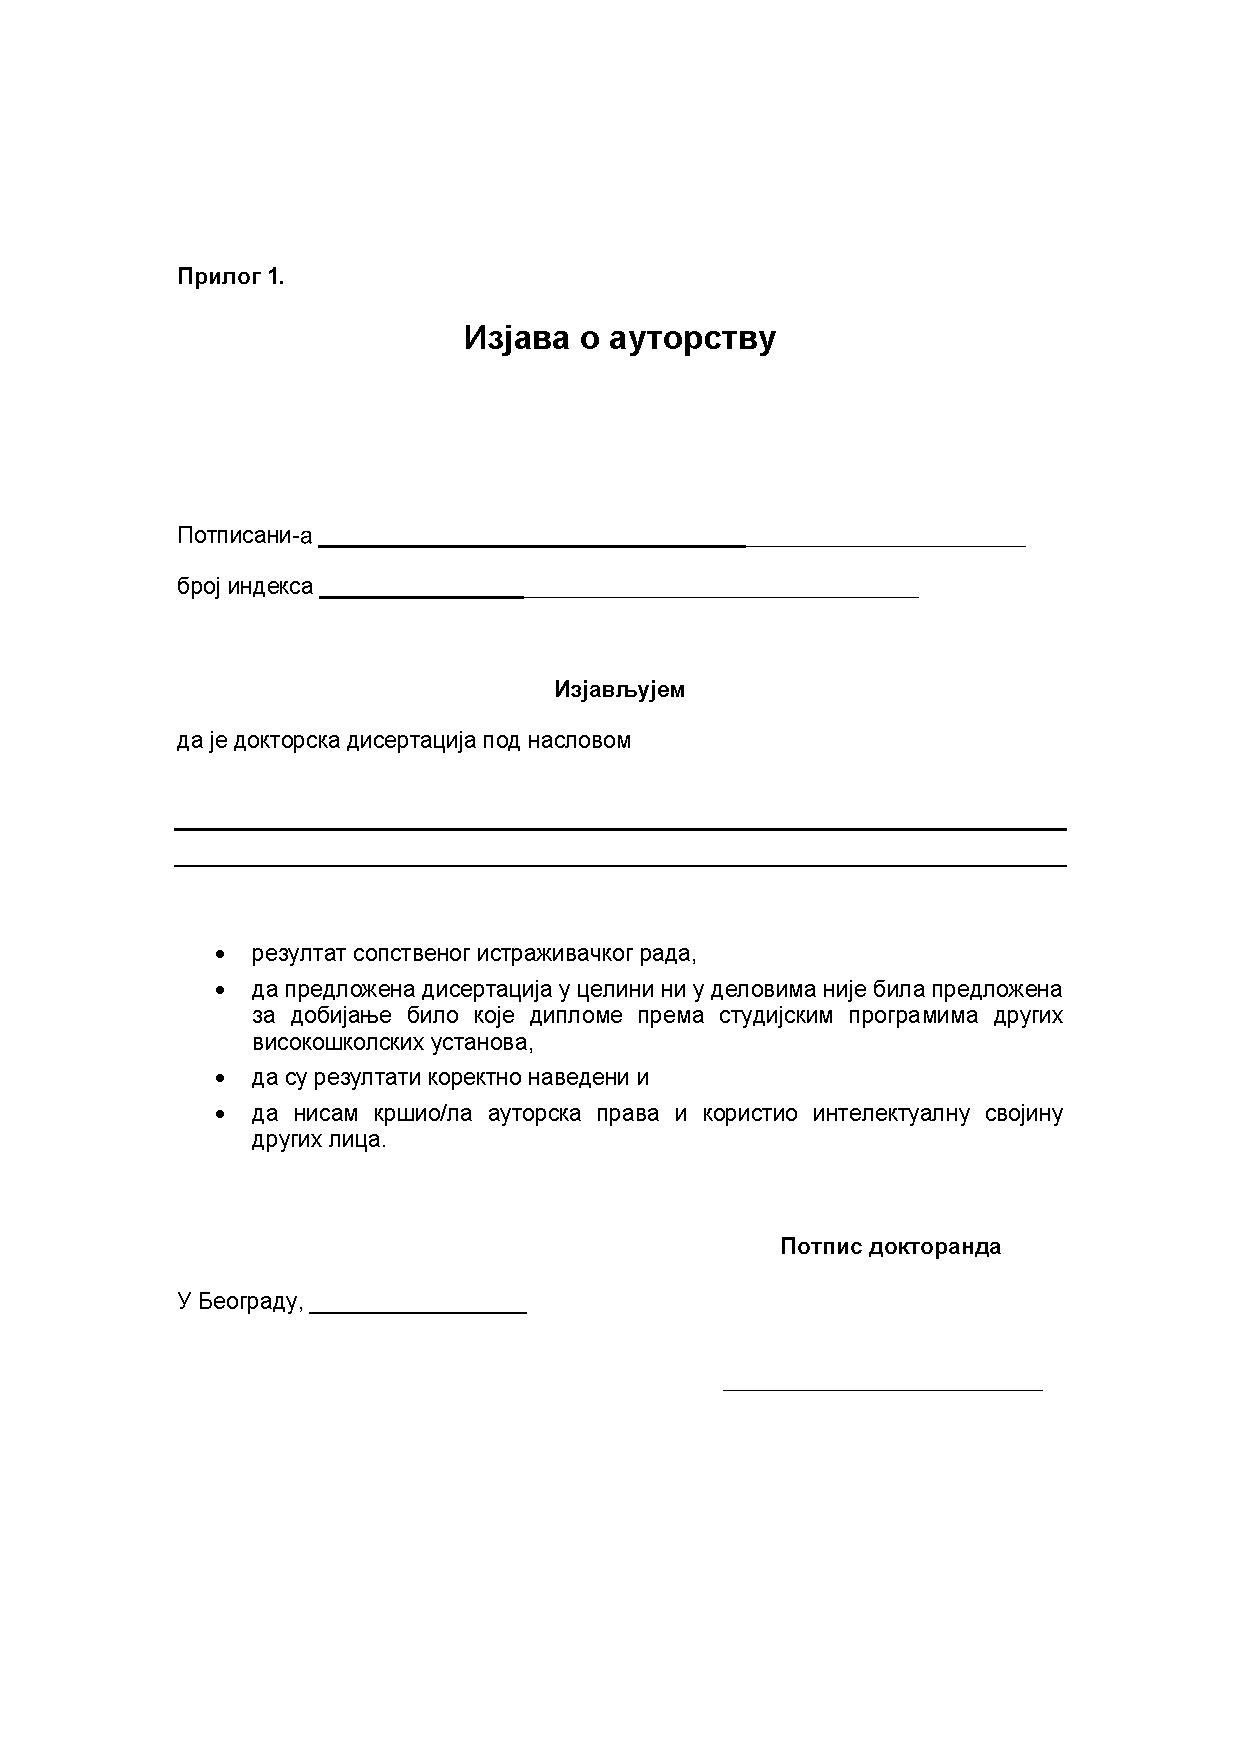
\includepdf{_Prilog1.pdf}
% Prilog 2: Izjava o istovetnosti štampane i elektronske verzije doktorskog rada
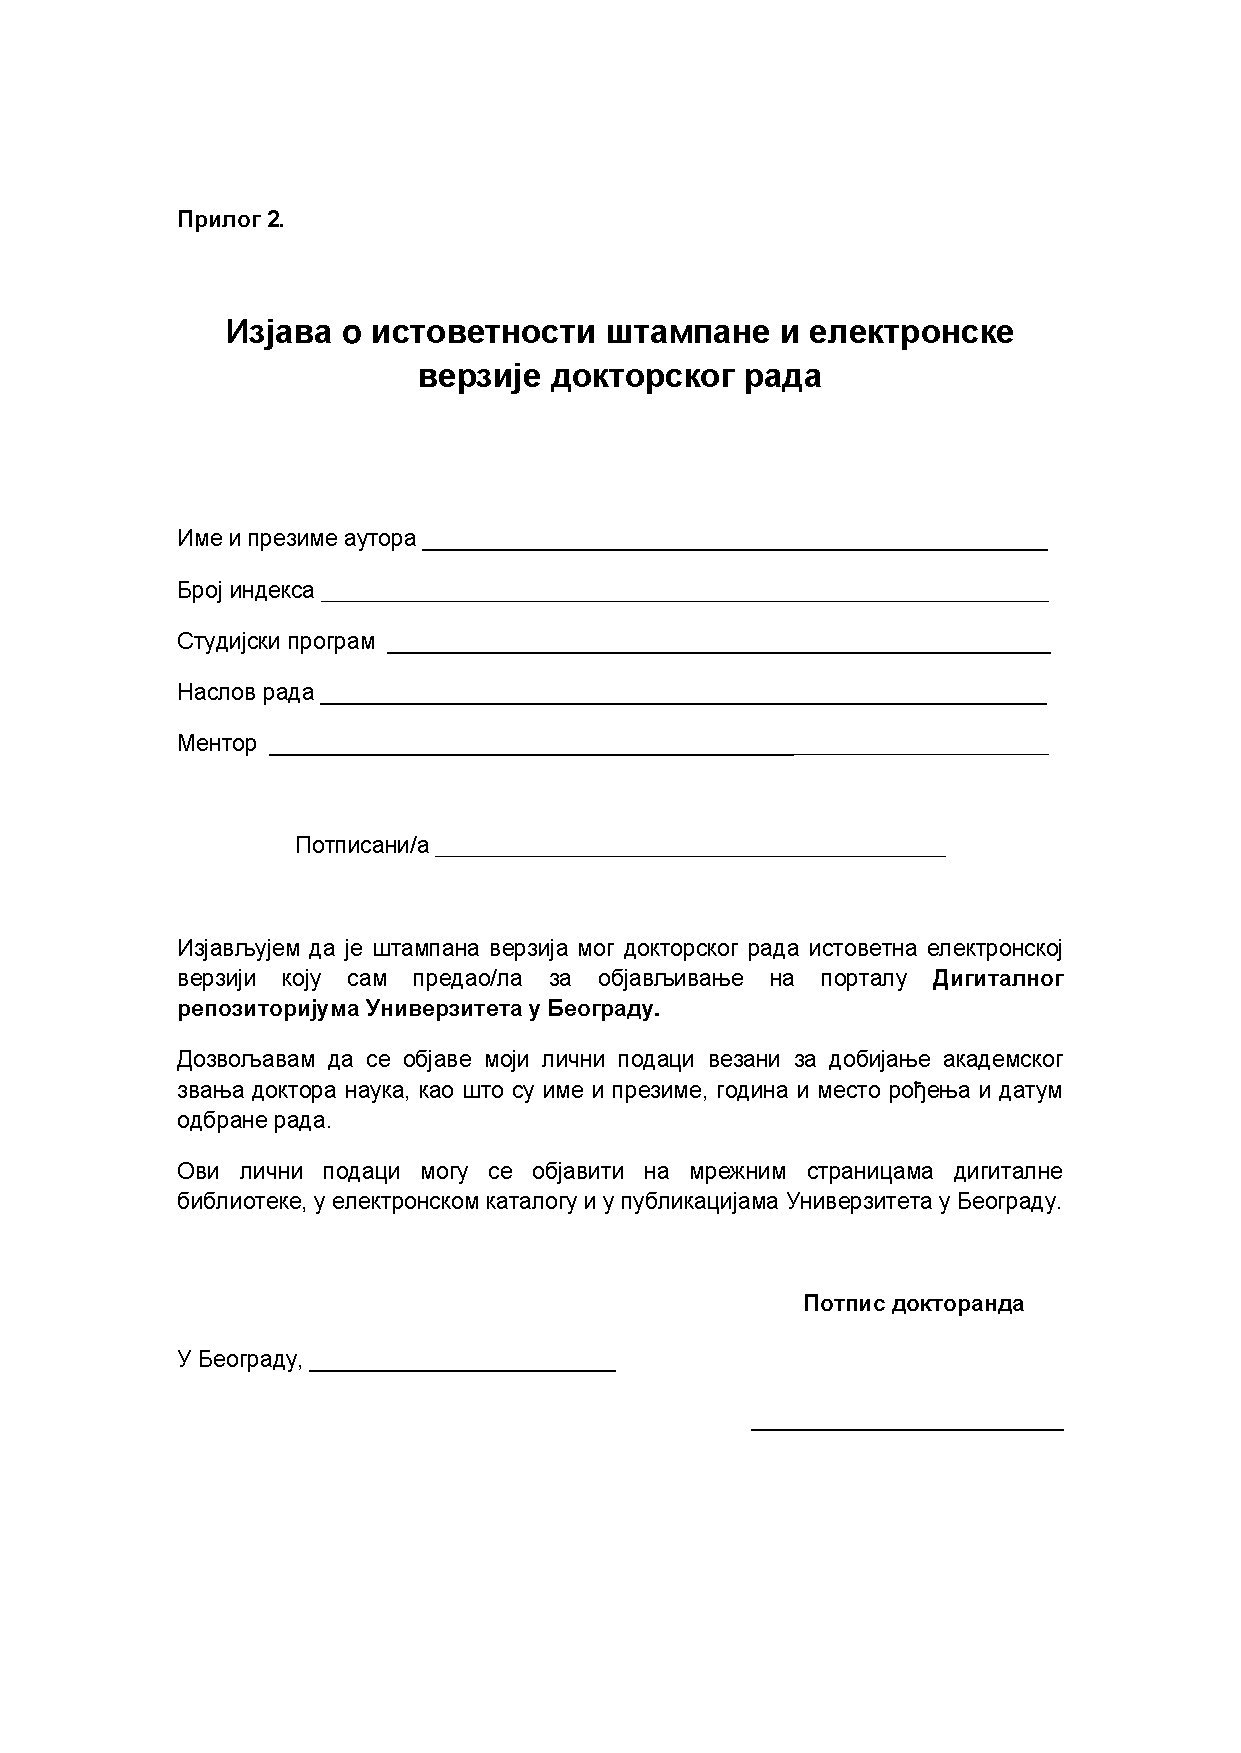
\includepdf{_Prilog2.pdf}
% Prilog 3: Izjava o korišćenju
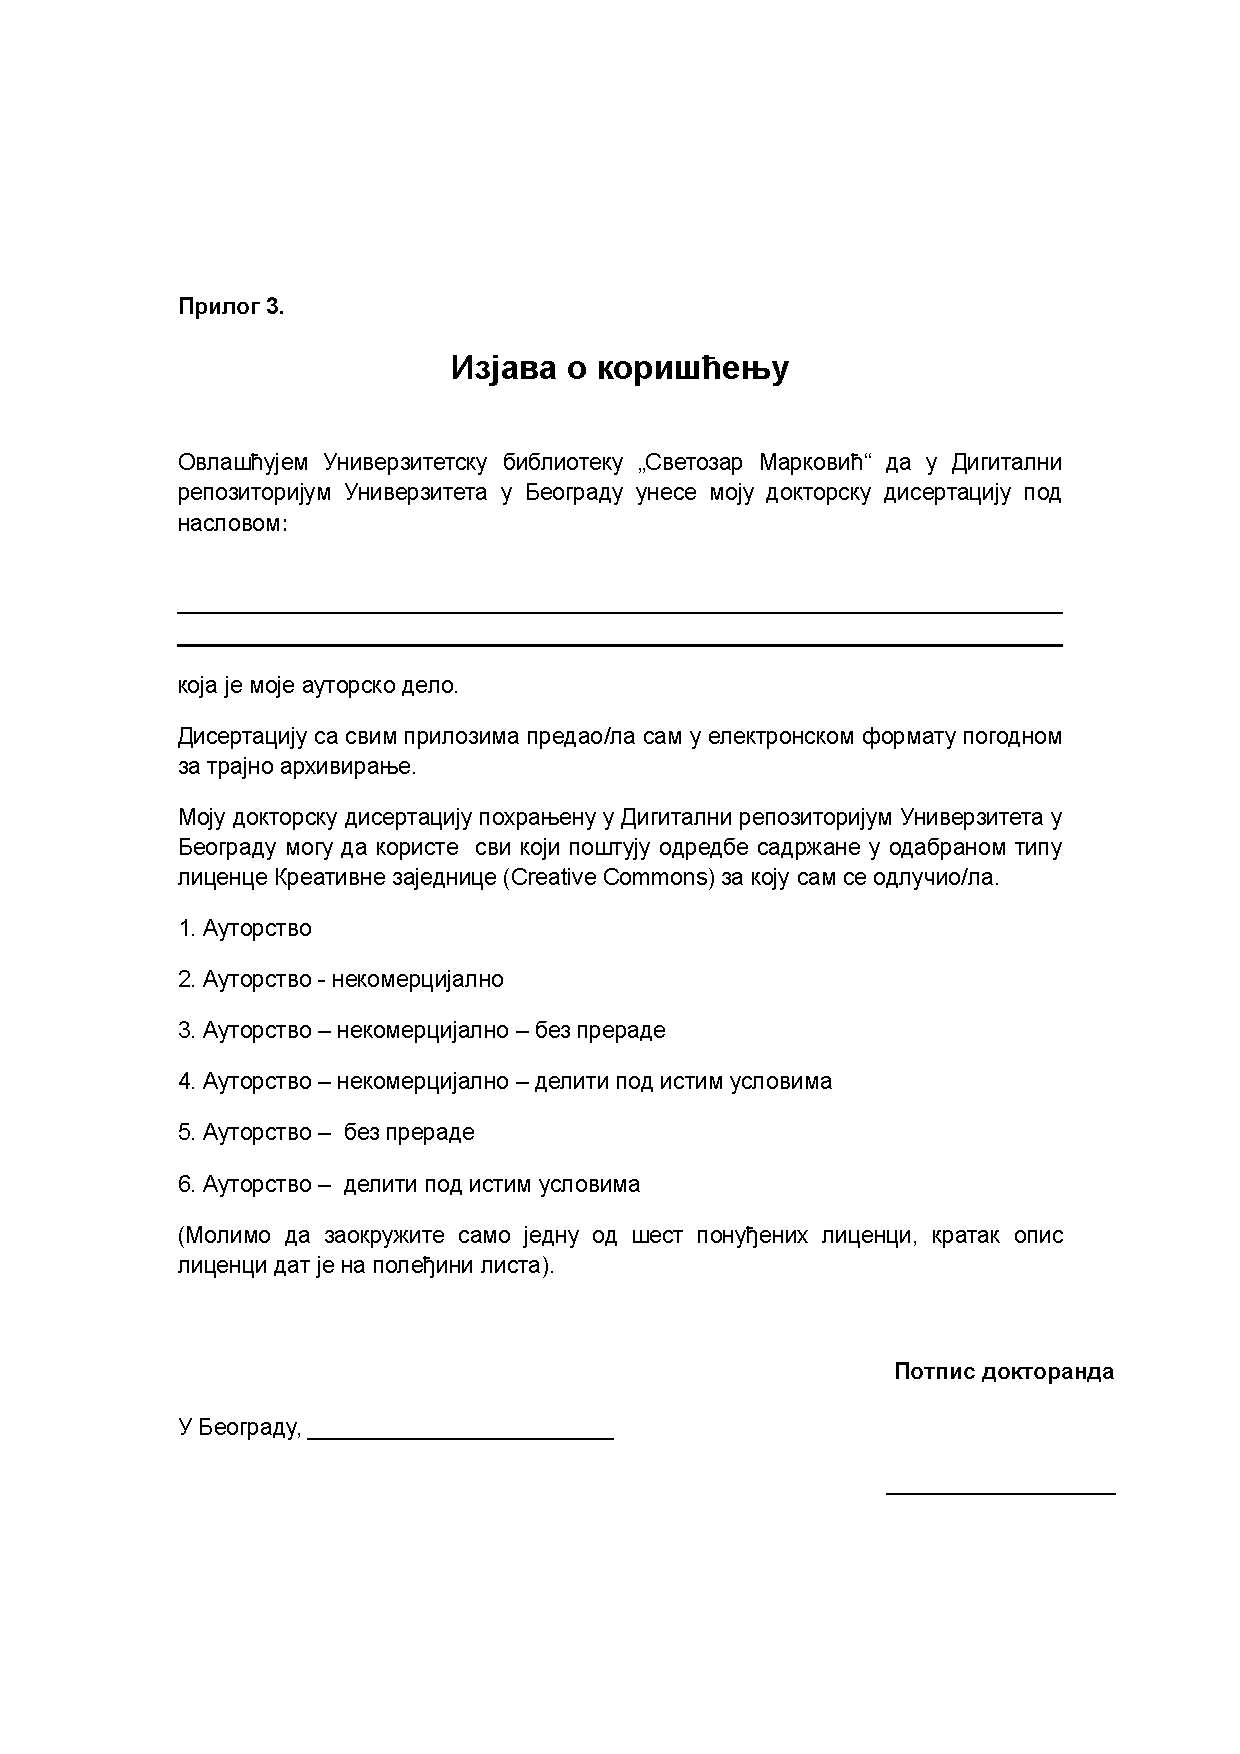
\includepdf{_Prilog3.pdf}

\end{document} 
